\documentclass[12pt, a4paper]{article}
\usepackage[utf8]{inputenc}
\usepackage{indentfirst} %indentace prvního odstavce
\usepackage{url}
\usepackage{amsmath}
\usepackage{graphicx}
\graphicspath{ {doc-img/} }

\title{OOP Zápočtový program - Diskrétní simulace metra}
\author{Jan Oupický}
\date{2018}

\begin{document}
\maketitle

\section{Zadání}

Program má za úkol provést diskrétní simulaci metra. Cílem této simulace bude zjištění doby cesty ze stanice A do stanice B za různých podmínek jako kapacita souprav, počet lidí, počet souprav apod. 

\section{Uživatelský manuál}

Spolu s programem je distibuován soubor \url{stanice.txt}, ve kterém je seznam stanic metra. Základně je v něm seznam stanic pražského metra v požadovaném formátu.

Uživatel si ale může tento soubor upravit podle libosti, akorát musí dodržet následující syntaxi:

\begin{itemize}
    \item Prázdné řádky jsou ignorovány.
    \item Řádek, který začíná "\#" je komentář. Tento řádek je také ignorován
    \item Na každém řádku se může nacházet pouze jedna stanice metra.
    \item Řádek se stanicí musí mít následujicí formát:
    \[ % hack pro posunuti doleva
    \displayindent0pt
    \displaywidth\textwidth
    \mathtt{[pismeno], [nazev], [km], [je\;konecna], [je\;prestupni], [prestupni\;pismeno]}\text{, kde}
    \]
    \texttt{[pismeno]} = Písmeno linky, na které se daná stanice nachází\\
    \texttt{[nazev]} = Název stanice\\
    \texttt{[km]} = Na kolikátém kilometru od počáteční stanice se stanice nachází. Počáteční stanice má 0. kilometr. Číslo může být i s desetinnou tečkou.\\
    \texttt{[je konecna]} = Zda je stanice konečná. 0 = ne, 1 = ano. Tento údaj není povinný (defaultně je 0)\\
    \texttt{[je prestupni]} = Zda je stanice přestupní. 0 = ne, 1 = ano. Tento údaj není povinný (defaultně je 0)\\
    \texttt{[prestupni pismeno]} = Písmeno linky, na kterou lze z dané stanice přestoupit. Tento údaj není povinný, pokud je předchozí údaj 0.\\
    Řádky mohou tedy vypadat např. takto:
    \begin{verbatim}
    C, Háje, 0, 1
    B, Českomoravská, 6.4
    B, Florenc, 10.9, 0, 1, C
    \end{verbatim}
\end{itemize}

Poté již stačí program spustit a vybrat počáteční a konečnou stanici. Uživatel může dále měnit více specifická nastavení:
\begin{itemize}
    \item "Čas přichodu": Kdy dorazíme do počáteční stanice od prvního výjezdu souprav. První soupravy totiž vyjedou v čase 0 z konečných stanic. Zbylé soupravy vyjíždějí po 5 minutových intervalech.
    \item "Hustota lidí": Kolik lidí příjde každou minutu do metra (každý do náhodné stanice).
    \item "Linka": Výběr linky, pro kterou chceme měnit další nastavení.
    \item "Rychost soupravy": Rychlost souprav na dané lince v kilometrech za minutu.
    \item "Počet souprav": Počet souprav na dané lince. Počet souprav je sudý, jelikož soupravy vyrážejí po párech z konečných stanic.
    \item "Kapacita soupravy": Kolik lidí se vejde do jedné soupravy.
    \item "Doba čekání ve stanici": Jak dlouho souprava čeká ve stanici v minutách.
\end{itemize}

Hodnoty "Hustota lidí" a "Kapacita soupravy" by měly být upraveny oproti reálným hodnotám. Například v pražském metru ve špičce příjde do metra cca 1200 lidí za minutu. Každá souprava má kapacitu zhruba 1400. Základní nastavení je odvozeno od těchto údajů. Nechceme simulovat všech 1200 různých lidí za minutu ale stačí nám zhruba $\frac{1}{20}$, tedy "Hustota lidí" = 50 a "Kapacita soupravy" = 70.

Po nastavení stačí stisknout tlačítko "Simuluj" a počkat na výsledek, který se objeví pod tlačíkem. Uživatel po skončení jedné simulace může změnit nastavení a simulaci opakovat opětovným stiskem tlačítka.
\begin{figure}[h]
\centering
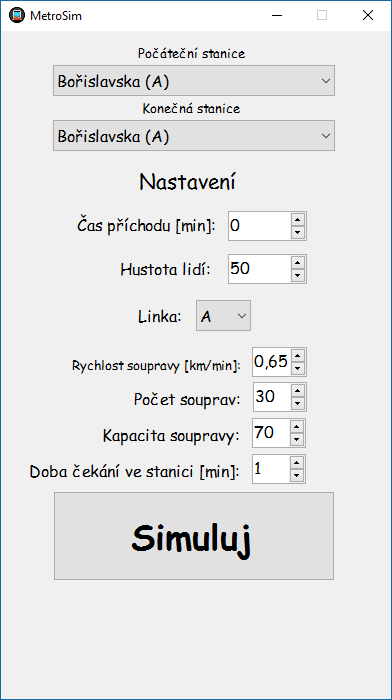
\includegraphics[scale=0.5]{obr1}
\caption{GUI programu}
\end{figure}

\section{Jak program funguje (algoritmus)}

Program je vlastně obyčejná diskrétní simulace, tudiž algoritmus velice jednoduchý na vysvětlení. Zhruba funguje takto:

\begin{itemize}
    \item Simulujeme jízdu souprav mezi stanicemi. Soupravy vyrážejí z konečných stanic po párech na každé lince v čase 0. Pokud je na lince více souprav (což je obvyklý případ), tak další pár vyráží po 5 minutách.
    \item Každou minutu nagenerujeme "Hustota lidí" počet lídí, kteří pojedou z náhodné stanice A do náhodné stanice B.
    \item V čase "Čas příchodu" vytvoříme hlavního pasažéra, který bude absolvovat trasu dle nastavení.
    \item Každý pasažér se snaží co nejkratší cestou dostat do své cílové stanice. Cestu má určenou tímto algoritmem:
        \begin{enumerate}
            \item Pokud je cílová stanice na stejné lince jako aktuální stanice, kde se pasažér nachází, tak pasažér nastoupí do soupravy, která jede správným směrem, a nevystoupí dokud nedorazí do cíle.
            \item Pokud neplatí 1., tak pasažér dojede do nejbližší přestupní stanice na danou linku, na které se nachází cílová stanice. Poté pokračuje krokem 1.
        \end{enumerate} 
    \item Simulace končí, když hlavní pasažér dorazí do cílové stanice.
\end{itemize}

Jelikož je generování ostatních pasažérů náhodné (odkud kam jedou), tak se výsledky různých simulací mohou výrazně lišit. Proto program provede v základním nastavení 16 simulací se stejným nastavením a zprůměruje výsledek.

\section{Implementace}

Skoro každá diskrétní simulace se skládá ze 4 hlavních tříd (\texttt{Udalost}, \texttt{Kalendar}, \texttt{Model}, \texttt{Proces}). Postupně si je všechny probereme. 

\subsection{Třída \texttt{Udalost}}
Tato třída v sobě neobsahuje žádnou logiku programu. Obsahuje v sobě pouze informace o dané události v simulaci. Tyto infomace jsou uloženy ve 3 promměných:
\begin{itemize}
    \item \texttt{int kdy}: Kdy se daná událost stane.
    \item \texttt{Proces kdo}: Který proces tuto událost zpracuje.
    \item \texttt{TypUdalosti co}: Identifikátor typu události. \texttt{TypUdalosti} je \texttt{enum}.
\end{itemize}

V programu se vyskytují tyto typy událostí (obsah \texttt{TypUdalosti}):
\begin{itemize}
    \item \texttt{prichodDoStanice}: Tato událost je zpracována třídou \texttt{Pasazer} (o ní později). Označuje událost, když pasažér příjde do stanice metra.
    \item \texttt{prijezdDoStanice}: Tato událost je zpracována třídou \texttt{Souprava} (o ní později). Označuje událost, když souprava přijede do stanice metra.
    \item \texttt{vyjezdZeStanice}: Tato událost je zpracována třídou \texttt{Souprava} (o ní později). Označuje událost, když souprava odjiždí ze stanice metra.
    \item \texttt{spawnSouprav}: Tato událost je zpracována třídou \texttt{Spawner} (o ní později). Označuje událost, kdy vyráží nové soupravy metra z konečných stanic.
\end{itemize}

\subsection{Třída \texttt{Kalendar}}
Třída \texttt{Kalendar} je také vcelku malá jednoduchá třída. Stará se pouze o uchovávání výše zmíněných událostí a slouží jako interface pro práci s tímto seznamem.

Seznam událostí je realizován třídou \texttt{List<Udalost>}. Pro manipulaci s kalendářem existují metody \texttt{void pridejUdalost(Udalost udalost)}, \texttt{Boolean jePrazdny()} a \texttt{Udalost vratNejaktulanejsi()}. Co tyto metody dělají snad plyne z názvu. Jediná otázka může nastat ohledně toho, co je to "nejaktuálnější" událost. Nejaktuálnější událost je ta, která má nejnižší hodnotu \texttt{cas}. Pokud je více takových, tak se vybere ta s nejnizším indexem v seznamu.

\subsection{Třída \texttt{Proces}}
Tato abstraktní třída je předkem všech tříd, které zpracovávají události. Obsahuje pouze 2 veřejné proměnné:
\begin{itemize}
    \item \texttt{string id}: identifikátor procesu
    \item \texttt{Model model}: odkaz na třídu \texttt{Model} (o ní později).
\end{itemize}

Poslední součást této třídy je abstraktní metoda \texttt{void zpracuj(Udalost udalost)}.

V programu se používají pouze 3 třídy, jejižch předkem je třída \texttt{Proces}.

\subsubsection{Třída \texttt{Souprava}}
Jak již plyne z názvu třídy, toto je třída pro soupravu metra. Obsahuje informace o rychlosti, kapacitě, lince, aktuální stanici apod. dané soupravy. Obsahuje metody:
\begin{itemize}
    \item \texttt{void jedDoDalsiStanice()}: Tato metoda spočítá dobu jízdy do následující stanice a vytvoří novou událost \texttt{prijezdDoStanice}.
    \item \texttt{void vystupovani()}: Tato metoda naplánuje událost \texttt{prichodDoStanice} příslušným pasažérům.
    \item \texttt{void nastupovani()}: Tato metoda přidá do seznamu příslušné pasažéry, pokud je volné místo.
    \item \texttt{void zpracuj(Udalost udalost)}: Tato metoda zpracovává 2 typy událostí:
    \begin{itemize}
        \item \texttt{prijedzDoStanice}: Zavolá metodu \texttt{void vystupovani()} a naplánuje událost \texttt{vyjezdZeStanice}.
        \item \texttt{vyjezdZeStanice}: Zavolá metody \texttt{void nastupovani()} a \texttt{void jedDoDalsiStanice()}.
    \end{itemize}
\end{itemize}

\subsubsection{Třída \texttt{Pasazer}}
Asi druhá nejhlavnější třída (po třídě \texttt{Model}) v celém programu co se týče samotného provedení simulace. Obsahuje informace a metody o příslušném pasažérovi (například aktuální stanici). Důležité metody jsou 2:
\begin{itemize}
    \item \texttt{void setPristiStanice()}: Pomocí výše zmíněného algoritmu nastaví pasažérovi jeho příští stanici.
    \item \texttt{void zpracuj(Udalost udalost)}: Tato metoda zpracovává pouze jednu událost \texttt{prichodDoStanice}. Zjistí, jestli aktuální stanice je konečná. Pokud ano, tak smaže pasažéra, pokud ne, tak zavolá metodu \texttt{void setPristiStanice()}. Poté ještě zjistí, zda se pasažér nachází na přestupná stanici. Pokud ano, tak naplánuje novou událost \texttt{prichodDoStanice} do druhé přestupní stanice za určitou dobu, která je určena parametrem \texttt{DOBA\_PRESTUPU} ve třídě \texttt{StaniceLoader} (o ní později). Pokud ne, tak zavolá metodu \texttt{void zaradNaNastupiste(Pasazer p, Stanice pristiStanice)}, která je metodou třídy \texttt{Stanice} (také později).
\end{itemize}

\subsubsection{Třída \texttt{SpawnerSouprav}}
Tato třída je vytvořená pouze z hlediska jednoduché implementace spawnování (vytváření) nových souprav. Pouze implementuje metodu \texttt{void zpracuj(Udalost udalost)}, která zpracovává pouze událost \texttt{spawnSouprav}, při níž pouze volá metodu \texttt{void spawniCastSouprav()} třídy \texttt{Model}.

\subsection{Třída \texttt{Model}}

\end{document}